% \documentclass{sigplanconf}
% \documentclass{sig-alternate}
\documentclass{acm_proc_article-sp}
\newcommand{\punt}[1]{}
%%
\newcommand{\footnotenonumber}[1]{{\def\thempfn{}\footnotetext{\small #1}}}
%%  
\usepackage{graphicx}
%\usepackage{times}
\usepackage{subfigure}
\usepackage{url}
\urlstyle{rm} % use roman instead of tt for URLs

\usepackage{listings}
\usepackage{amsmath}
\usepackage{amsfonts}
\usepackage{amssymb}

\newtheorem{thm}{Theorem}
\newtheorem{prop}[thm]{Proposition}
\newtheorem{cor}[thm]{Corollary}
\newtheorem{lem}[thm]{Lemma}
\newtheorem{defn}[thm]{Definition}

\newcommand{\cfunction}[1]{{\bf \tt #1}}
\newcommand{\malloc}{\cfunction{malloc}}
\newcommand{\realloc}{\cfunction{realloc}}
\newcommand{\free}{\cfunction{free}}
\newcommand{\madvise}{\cfunction{madvise}}
\newcommand{\brk}{\cfunction{brk}}
\newcommand{\sbrk}{\cfunction{sbrk}}
\newcommand{\mmap}{\cfunction{mmap}}
\newcommand{\munmap}{\cfunction{munmap}}
\newcommand{\mprotect}{\cfunction{mprotect}}
\newcommand{\mlock}{\cfunction{mlock}}

\hyphenation{app-li-ca-tion}
\hyphenation{Die-Hard}
\hyphenation{Archi-pe-la-go}
\hyphenation{buf-fer}

\lstset{language=c++, basicstyle=\ttfamily,frame=single,numbers=left,numberstyle=\tiny,tabsize=4}

\begin{document}

%\conferenceinfo{ASPLOS XIII}{March 1-5, 2008, Seattle, WA}

% \title{Archipelago: Probabilistic Object-Level Isolation}
%\title{Archipelago: Object Islands in a 64-Bit Ocean}
\title{Archipelago: Trading Address Space \\ for Reliability and Security}
\numberofauthors{1} 
\author{
% 1st. author
\alignauthor
Vitaliy B. Lvin, Gene Novark, Emery D. Berger, Benjamin G. Zorn$^\dag$ \\
{\center \hspace{5em}	\affaddr{Dept. of Computer Science} \hfill \affaddr{$^\dag$Microsoft Research} \hspace{5em} } \vspace{-0.4em} % \\
{\center \hspace{5em}	\affaddr{University of Massachusetts} \hfill \affaddr{One Microsoft Way} \hspace{5em} } \vspace{-0.4em} % \\
{\center \hspace{5em}	\affaddr{Amherst, MA 01003} \hfill \affaddr{Redmond, WA 98052} \hspace{5em} } \vspace{-0.4em} % \\
}
% \date{27 June 2007}

\maketitle

\begin{abstract}
Memory errors are a notorious source of security vulnerabilities that
can lead to service interruptions, information leakage and
unauthorized access. Because such errors are also difficult to debug,
the absence of timely patches can leave users vulnerable to attack for
long periods of time. A variety of approaches have been introduced to
combat these errors, but these often incur large runtime overheads and
generally abort on errors, threatening availability.

This paper presents Archipelago, a runtime system that takes advantage
of available address space to substantially reduce the likelihood that
a memory error will impact program execution. Archipelago randomly
allocates heap objects far apart in virtual address space, effectively
isolating each object from buffer overflows. Archipelago also protects
against dangling pointer errors by preserving the contents of freed
objects after they are freed. Archipelago thus trades \emph{virtual}
address space---a plentiful resource on 64-bit systems---for
significantly improved program reliability and security, while
limiting
\emph{physical} memory consumption by tracking the working set of an
application and compacting cold objects. We show that Archipelago
allows applications to continue to run correctly in the face of
thousands of memory errors. Across a suite of server applications,
Archipelago's performance overhead is 6\% on average (between -7\% and
22\%), making it especially suitable to protect servers that have
known security vulnerabilities due to heap memory errors.
\end{abstract}

% A category with the (minimum) three required fields
%\category{D.3.3}{Programming Languages}{Dynamic storage management}
%\category{D.2.0}{Software Engineering}{Protection mechanisms}
%\category{G.3}{Probability and Statistics}{Probabilistic algorithms}

%\terms{Algorithms, Languages, Reliability}

%\keywords{Archipelago, randomization, dynamic memory allocation, probabilistic memory safety}

\section{Introduction}
\label{sec:intro}

\noindent
Memory errors in C and C++ programs continue to be a significant
problem. They are hard to debug and often easy to
exploit. Memory-based attacks are an effective way to compromise
Internet servers, either by crashing them, which causes service
interruptions and data loss, or by making them execute arbitrary
code. Because these bugs are difficult to debug, it can take weeks
before even critical errors are repaired~\cite{symantec}, leaving
applications vulnerable to attack.
 
A variety of approaches have been developed to help programmers avoid
memory errors. These approaches can be roughly classified into three
categories: testing tools, garbage collectors, and compiler-based
tools. Testing tools, such as
Valgrind~\cite{Net:bounds-checking2004,Sew:memcheck2005} and
Purify~\cite{Hastings:91}, impose performance overheads that only make
their use feasible during testing. Conservative garbage
collectors~\cite{boeh88} only protect against dangling pointer errors
and provide no protection against buffer overflows. Compiler-based
approaches~\cite{178446,1062520,da06icse,1133999,713871,503286,cred,1029913,940113}
typically incur unacceptably-large runtime overheads or require
programmer intervention, and also require source code, which may not
be available. They also generally abort program execution in response
to memory errors, reducing availability and leaving systems vulnerable
to denial-of-service attacks.

%
 
%The majority of these approaches aim to assign sound fail-stop semantics to erroneous programs: as soon as the program execution triggers a memory error, it is terminated. Rinard et al.~\cite{bmb} attempt to preserve program semantics and allow execution through buffer overflow errors, but their system design has inherent limits on the size of buffer overflows it can tolerate while maintaining soundness. Moreover, it doesn't provide any protection against dangling pointer errors.

\noindent
{\bf Contributions:} This paper presents Archipelago, a runtime system
that significantly improves the resilience of applications to
heap-based memory errors.\footnote{\small An \emph{archipelago} is an
expanse of water with many scattered islands, such as the Aegean Sea.}
Archipelago treats heap objects as individual islands, surrounded by
stretches of unused address space. On modern architectures,
especially 64-bit systems, virtual address space is a plentiful
resource.  Archipelago trades this plentiful resource for a high
degree of \emph{probabilistic memory safety}~\cite{1134000}; in other
words, Archipelago can use available \emph{virtual} memory to significantly
increase the likelihood that a program will run correctly in the face
of memory errors.

To control \emph{physical} memory consumption, Archipelago leverages
the following key insight: once the distance between objects crosses a
certain threshold, each page will hold exactly one (small) object. At
this point, additional address-space expansion is free: the virtual
memory system does not need to allocate physical frames for unused
address space between objects. Archipelago takes advantage of this
insight and directly allocates one object per page, leaving the
virtual address space between objects uncommitted. It further limits
physical memory consumption by selectively compacting pages of the
heap that are infrequently used.

The class of applications that are most sensitive to memory errors and
associated security vulnerabilities are servers: they are attractive,
high-value targets that are connected directly to the Internet. We
show that Archipelago can provide high levels of safety and
reliability for this class of applications. We show that Archipelago
can let applications run even in the face of thousands of memory
errors, while keeping performance impact to acceptably-low
levels. Archipelago slows down execution of a range of server
applications by just 6\% on average (from -7\% to 22\%). This modest
performance impact makes Archipelago a realistic approach to protect
deployed server applications against known and unknown heap-based
security vulnerabilities.

While the primary focus of this work is using available memory to
increase the availability and security of networked server
applications, Archipelago can also \emph{detect} memory errors. In
this mode, Archipelago is both more efficient and more thorough than
standard memory debugging tools. Because it generally allows programs
to run despite memory errors, it can detect multiple heap overflows in
a single execution, rather than halting on the first error.

% FIX ME EDB Trades address space for reliability.
% FIX ME EDB committed versus mapped.

%Archipelago\ takes a different approach. While not completely sound, it provides \emph{probabilistic memory safety}---a probabilistic guarantee that memory errors will be benign during a program execution. Moreover, it can provide protection to unmodified, binary programs, without access to the source code and without prohibitive performance overhead, which makes it an ideal remedy for bugs in deployed servers while no bug fixes are available.

The rest of the paper is organized as follows. Section~\ref{sec:prob}
reviews operating system support for virtual memory, and explains
probabilistic memory safety. Section~\ref{sec:qih} describes the
software architecture of Archipelago in detail. Section~\ref{sec:eval}
evaluates the effectiveness of Archipelago at withstanding memory
errors and measures its overhead. Section~\ref{sec:efence}
describes how Archipelago detects buffer overflows, and compares its
use in this mode to two widely-used memory
debuggers. Section~\ref{sec:related} surveys related work,
Section~\ref{sec:future} discusses future directions, and
Section~\ref{sec:fin} concludes.

\section{Background}

\subsection{Virtual Memory}
\label{sec:virtual_memory}

\noindent
Because Archipelago makes extensive use of operating system support
for virtual memory management that may not be familiar, we define some
key terms and concepts here.

A key distinction is that between virtual and physical memory. Virtual
memory refers to the full addressable range of memory. This range does
not necessarily correspond to the architecture's word size---on x86-64
architectures, the addressable range is 48 bits (i.e., $2^{48}$
bytes). Operating systems map virtual memory to available physical
memory. On 64-bit systems, virtual memory is plentiful while physical
memory is in relatively short supply (e.g., on the order of 1--8
gigabytes ($2^{30}$--$2^{33}$) bytes).

Virtual memory is divided into pages that are typically 4K
chunks. Pages can be in three states: \emph{unmapped},
\emph{reserved}, and \emph{committed}. An unmapped page is not
available for use by the process, and access to it triggers a
segmentation violation.

When a process obtains a page from the system via {\tt mmap}, the
virtual address range is \emph{reserved} so that a subsequent call to
{\tt mmap} is guaranteed to return virtual memory from a different
range. However, a reserved page does not initially have an associated
physical page frame.

When a reserved page is touched for the first time, the page is
\emph{committed}: a physical page frame is allocated and associated with the
virtual page. The kernel initializes all page contents to zero when
they are first touched. Subsequent touches do not result in any page
faults unless, due to memory pressure, the page is
\emph{evicted} to disk. In this case, the page's contents are
generally written to the disk, and then the page is decommitted (but
remains reserved). A subsequent touch triggers a page fault, and the
kernel will fill the page with the contents previously saved on disk.

Operating systems allow programmers to control the state of pages via
the \madvise\ system call. A Unix application can invoke {\tt
madvise(MADV\_FREE)} to inform the kernel that a range of pages is
available to be reclaimed, and that there is no need to write the
contents to disk. This call thus decommits a page's physical frame,
making it available for reuse by the system. Archipelago makes use of
\madvise\ to limit its physical memory footprint, as Section~\ref{sec:allocator} describes. \madvise\ can also be used to provide hints to guide the virtual memory manager's page replacement algorithm, a feature that Archipelago also uses.

Additionally, an application can protect access to a page so that
accesses trigger a signal, even if the page has been committed. For
example, an application can invoke {\tt mprotect(...,PROT\_NONE)} on a
range of pages: future attempts to read, write, or execute memory on
this page will trigger a segmentation violation. By installing a
custom signal handler to handle these segmentation violations, an
application can selectively intercept reads or writes to particular
pages. Archipelago uses these memory protection calls to let it
perform compaction of cold objects (see Section~\ref{sec:compaction}).


% EDB - hot space?

\subsection{Probabilistic Memory Safety}
\label{sec:prob}

\noindent
The motivation for our work comes from the ideas of \emph{infinite
heaps} and \emph{probabilistic memory safety} originally introduced by
Berger and Zorn~\cite{1134000}.

An \emph{infinite heap memory manager} is an ideal,
unrealizable runtime system that allows programs containing memory
errors to execute soundly and to completion. In such a system, the
heap area is infinitely large and can never be exhausted. All objects
are allocated fresh, infinitely far away from each other, and are
never deallocated.

Because every object is infinitely far away from any other object,
buffer overflows become benign, and dangling pointers also vanish
since objects are never deallocated or reused. A portable correct C
program cannot tell the difference between an infinite heap memory
manager and a normal allocator, while a program containing memory
errors would execute correctly for reasons outlined above, as long as
it does not contain uninitialized reads.

Of course, it is impossible to build a true infinite heap memory
manager. However, one can approximate its behavior by using an
\emph{M-heap}---a heap that is \textit{M} times larger than
needed. By placing objects uniformly randomly across an
\textit{M}-heap, we get the expected minimum separation between any
two objects of \textit{M} -- 1 objects, and therefore overflows that
are smaller become benign with high probability. By
\emph{randomizing} the choice of freed objects to reuse, we minimize the
likelihood of recently freed objects being overwritten, and therefore
of a malignant dangling pointer error. This heap thus provides
\emph{probabilistic memory safety}, a probabilistic guarantee that
memory errors occurring in the program are benign during its
execution.

\newpage

In an \textit{M}-heap, the likelihood of no live objects being
overwritten by an overflow \textit{N} objects in size is
$(1-\frac{1}{M})^{N}$~\cite{1134000}.

Based on this formula, it is clear that one way to increase the
probability of correct execution in the presence of memory error is to
make the \emph{heap expansion factor} (M) large. For example,
\textit{M}~=~100 yields a 99\% probability that a buffer overflow
smaller or equal to the size of an object will be benign. It is
impractical, however, to run DieHard system with large values of
\textit{M} because of its correspondingly large physical memory
consumption (see Section~\ref{sec:eval}).

Archipelago achieves these probabilistic guarantees against buffer
overflows while consuming only a correspondingly large amount of
\emph{virtual} memory. It effectively controls physical memory
consumption and provides lower CPU overheads than a comparably-sized
DieHard heap, as Sections~\ref{sec:eval-runtime} and
\ref{sec:eval-memory} show.


\section{Archipelago Architecture}

\label{sec:qih}

\noindent
Archipelago consists of two parts: a randomizing memory allocator and
a cold storage module, which controls the overall physical memory
consumption of the program. These parts are compiled into a
dynamically-linked library that, when pre-loaded before an executable,
replaces standard memory management routines, such as \malloc\ and
\free, with calls to the Archipelago allocator.


\subsection{Object-Per-Page Allocator}
\label{sec:allocator}

\begin{figure}[!t]
\label{fig:malloc}
\begin{lstlisting}[frame=trbl]{}
void * malloc (size_t size) {
	if (size <= PAGE_SIZE) {
		//object fits on a page
		//obtain random page from the pool
		void *page = getRandomPage(); 
	}
	if (page == NULL) { 
		//object doesn't fit on the page
		//or pool is full
		//mmap memory directly
		void *pages = 
			mmap(roundUpToPageSize(size),
				  MAP_ANONYMOUS);
	}	
	if (page == NULL) {
		//mmap failed
		return NULL;
	}
	//add coloring 
	void *ptr = 
			getRandomColoring(page, size);
	//register page(s) as part 
	//of working set
	registerActivePages(page, ptr, size);
	return ptr;		
}
\end{lstlisting}
\caption{Pseudo-code for Archipelago's \malloc.}
\end{figure}

\begin{figure}[!t]
\label{fig:free}
\begin{lstlisting}[frame=trbl]{}
void free (void * ptr) {
	//retrieve  size
	size_t size = getObjectSize(ptr);
	//get first page
	void *page = getStartPage(ptr);
	//unregister pages being deleted
	unregisterActivePages(page, ptr, size);
	//discard pages 
	//that have been compacted
	discardCompactedPages(page, ptr, size);
	if (size <= PAGE_SIZE) { 
		//object fits on page:
		//discard contents
		madvise(page, MADV_FREE); 
	} else { 
		//object doesn't fit on page:
		//unmap it
		munmap(page, 
			roundUpToPageSize(size));
	}
}
\end{lstlisting}
\caption{Pseudo-code for Archipelago's \free.}
\end{figure}

\noindent
% {\bf FIX ME: EDB overview, then malloc, then hot/cold (forward ref), then free. Note that the current model is not adaptive.}

% {\bf FIX ME: where's the architecture diagram?}
Key to Archipelago's protection from memory errors is its
object-per-page memory allocator. It is constructed using the Heap
Layers infrastructure~\cite{BergerZornMcKinley:2001}. As implied by
its name, the object-per-page allocator places each allocated object
on a separate virtual memory page. It reserves (but does not commit) a
large fraction of the address space using \mmap, and uses it as a pool
from which to draw pages to satisfy allocation
requests. Figures~\ref{fig:malloc} and \ref{fig:free} present
pseudo-code for \malloc\ and \free.

The size of the pool of available pages is a parameter to Archipelago
(defaulting to 512 megabytes) that represents the trade-off between
the protection Archipelago provides and its virtual memory
consumption. A larger pool will provide more robust protection against
errors, but at the cost of increased virtual memory consumption. Note
that in case of memory pressure, the virtual memory manager will
reclaim all committed but unused pages in the pool first, making the
footprint of the application independent of the pool size. 

{\bf Allocation:} Objects are placed on pages randomly chosen from the
pool (Figure~\ref{fig:malloc}, line 5). The object-per-page allocator
uses a bit array to distinguish between used (allocated) and unused
pages in the pool, and probes in the bit array to perform this random
selection. In order to bound the expected number of probes to find an
empty page, the object-per-page allocator always keeps the pool no
more than half full. This strategy bounds the worst-case expected
number of probes to a small constant (2).

Notice that since pages in the pool are allocated randomly, no
locality of reference exists between pages in the pool. We give a hint
to the virtual memory manager that no locality exists and that it
should not prefetch pages within the pool using \madvise\ (not shown in
the code). Together with \mmap,
\madvise\ ensures that pages are not instantiated in the physical
memory until they are actually needed.

To reduce cache conflicts, Archipelago uses \emph{colors} to place
objects on pages: objects are placed at random offsets on pages,
taking care to keep objects within their pages' boundaries (lines
20--21). Coloring helps reduce L2 misses due to cache conflicts and
thus improves performance (we do not report these results here due to
space limitations).

{\bf Deallocation:} When an object smaller than a page in size is
deleted, the object-per-page allocator marks the page as
free (Figure~\ref{fig:free}, lines 5--10). Moreover, it instructs the virtual memory manager using
\madvise\ to discard the contents of the page without writing them to
disk, therefore reducing the overall runtime overhead of the system
due to page eviction (line 14).

{\bf Large objects:} Objects that do not fit on a single page are
treated specially by the object-per-page allocator. Archipelago
currently does not search for ranges of free pages in the pool but
instead allocates memory directly using \mmap\
(Figure~\ref{fig:malloc}, lines 7--13). When the memory pool gets more
than half full, all objects are allocated via \mmap to avoid costly
probes for free pages in the pool.

Because current Linux kernels randomize locations of memory-mapped
objects in the address space, the object-per-page allocator need not
take further action. When an object that was allocated using
\mmap\ is freed, its memory is immediately released back to the
operating system using \munmap (Figure~\ref{fig:free}, lines 18--19).

%\begin{figure}
%\label{fig:heap}
%\begin{center}
% 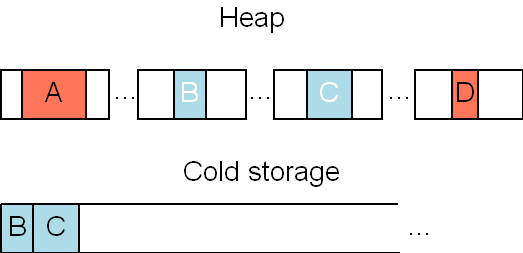
\includegraphics[height=1.2in]{heap.png}
% % heap.png: 523x253 pixel, 72dpi, 18.45x8.93 cm, bb=0 0 523 253
%\caption{Archipelago object layout.}
%\end{center}
%\end{figure}

\subsection{Exploiting Working Sets}
\label{sec:compaction}

\noindent
Running programs with the object-per-page allocator alone would
consume so much physical memory that it would be impractical for
deployed programs. In order to limit its physical memory consumption,
Archipelago relies on the observed temporal locality of memory
accesses in most programs, or the so-called \emph{working set
hypothesis}. A program at any given time has a
\emph{working set}, a (hopefully) small subset of all live objects on
which the program is actively operating.

The notion of a working set is extensively used in the virtual memory
managers~\cite{denn68}, which attempt to keep just the working sets of
running programs in memory while storing rarely used data in secondary
storage.

Archipelago follows a similar design: it tracks the working set of a
program, moves objects not in the working set into a more compact
representation, and returns the physical pages they occupied to the
OS.

Operating systems typically rely on hardware-managed dirty and
reference bits that give them precise information about which pages
are being used. While a similar approach can be implemented in
user-space with memory protection mechanisms, the cost of such an
approach would be prohibitively high compared to the cost of making a
mistake and compacting a page that is in the working set.

Instead, Archipelago uses a cheap approximation of the working
set. Archipelago keeps all the pages occupied by live objects in a
bounded FIFO queue. In our current implementation, the size of the
FIFO queue is fixed at startup time, either read in from an
environment variable or defaulting to 5000 objects. Pages are added to
the back of the queue at allocation time. As the queue becomes full,
pages at the front of the queue are removed and compacted. Upon access
to a compacted page, the page is restored and added to the end of the
queue as well.

\subsection{Cold Storage}
\label{sec:cold}

\begin{figure}[!t]
\label{fig:compact}
\begin{lstlisting}
void deflate (void *page) {
	// allocate space in cold store
	void *coldStore = coldHeap.malloc(
		hotPages[page]->getDataSize());
	// move the data
	memcpy(coldStore, 
		hotPages[page]->getDataStart(), 
		size);
	// return physical page to OS
	madvise(page, MADV_FREE);
	// set trap on future accesses
	mprotect(page, PROT_NONE);
	// mark page as cold
	coldPaged[page] = hotPages[page];
	hotPages.remove(page);
	// remember the location of the data
	coldPages[page].
		setColdStore(coldStore);
}

bool inflate (void *page) {
	// check page was deflated before
	if (!coldPages.hasKey(page))
		return false;
	// enable access to the page
	mprotect(page, PROT_READ | PROT_WRITE);
	// restore data
	memcpy(coldPages[page].getStart(),
		coldPages[page].getColdStore(),
		coldPages[page].getSize());
	// free the cold space
	coldHeap.free(
		coldPages[page].getColdStore());
	// mark page as hot
	hotPages[page] = coldPages[page]
	coldPages.remove(page);
	return true;
}

void sigsegv_handler(void *addr) {
	if (!inflate(getPageStart(addr))) {
		fprintf(stderr, "Overflow!\n")
		exit(-1);
	}
} 
\end{lstlisting}
\caption{Pseudo-code for Archipelago's compaction and uncompaction routines.}
\end{figure}

\noindent
Archipelago contains functionality that compacts pages not in the
current working set, thus reducing its physical memory
requirements. It uses an in-memory compaction mechanism that stores
compacted objects in a separate heap managed by the general-purpose
Lea allocator~\cite{lea97}.

When a page is compacted, its non-zero contents are copied out into
this internal heap. Then, any accesses to the page are disabled by
\mprotect, so that Archipelago receives a protection violation signal
the next time the application tries to access the page. Finally, the
virtual memory manager is instructed using
\madvise\ not to write the page contents to disk.

Archipelago installs a custom signal handler to receive protection
violation signals and restore objects back from cold storage. When the
handler receives a signal, it first checks whether the application was
trying to access a page in cold storage. If it was, the handler has to
restore that page in order for the application to continue. The
handler unprotects the page and restores the data on it from cold
storage. It also places the page back on the queue of active pages,
and frees the space used to hold the page's data in cold
storage. Control then passes back to the application, which can now
safely continue.

%Figure~\ref{fig:state-diag} shows the overall life cycle of a page and
%which component of the system is managing it.

While compacting pages imposes additional runtime overhead, it
effectively controls physical memory overhead, as
Section~\ref{sec:eval-memory} shows.

%\begin{figure}
% \centering
% 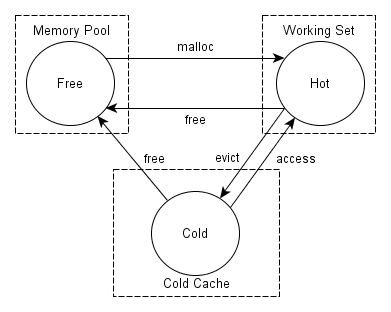
\includegraphics[height=1.8in]{page-state-diagram.png}
% % mockhist.png: 591x436 pixel, 80dpi, 18.77x13.85 cm, bb=0 0 532 392
% \caption{Life cycle of a page.}
% \label{fig:state-diag}
%\end{figure}

\section{Evaluation}
\label{sec:eval}

\noindent
In our evaluation, we answer the following questions:

\begin{enumerate}
\item What is the runtime overhead of using Archipelago with server applications?
\item What is the memory overhead of using Archipelago with server applications?
\item How effective is Archipelago against both injected faults and real errors?

\end{enumerate}
\subsection{Experimental Methodology}


\noindent
We perform our evaluation on a quiescent dual-processor with 8
gigabytes of RAM. Each processor is a 4-core 64-bit Intel Xeon running at
2.33 Ghz and equipped with a 4MB L2 cache.

We compare Archipelago to the GNU C library, which uses a variant of
the Lea allocator~\cite{lea97}, and to DieHard, version 1.1. This
version, available from the project website, is an adaptive variant
that dynamically grows its heap~\cite{berg07}, and so is more
space-efficient than the original, published
description~\cite{1134000}.

One important caveat is that we run all experiments on a particular
version of a recent Linux kernel, version 2.6.21-mm2. This kernel
version uses a more sophisticated algorithm for managing physical
memory pages that were initially used by applications, but then
returned to the kernel. This \emph{page laundering} process updates a
number of kernel data structures and potentially writes the page's
contents to secondary storage. Linux kernel versions up to and
including 2.6.21 launder pages \emph{eagerly} whenever an application calls
\madvise. However, Linux version 2.6.21-mm2 launders pages \emph{lazily}, waiting until
more physical memory pages are actually needed. In the absence of
memory pressure, this policy improves our system's performance on an
allocation-intensive microbenchmark by a factor of two: \madvise\ is
on Archipelago's normal deallocation path. Because of its performance
advantages for ordinary workloads, we expect that this patch, or one
similar to it, will be adopted in future versions of the Linux kernel.

\subsection{Performance Overhead}
\label{sec:eval-runtime}

\noindent
To quantify the performance overhead of using Archipelago, we measure
the performance of a range of server applications running with and
without Archipelago. All observed variances were below 1\%. In our
experiments, Archipelago uses a memory pool 512MB in size. We also
compare performance against DieHard with two different heap multiplier
values: 2 and 1024. The first multiplier provides performance and
protection similar to the results reported in the original DieHard
paper, while the second multiplier more closely approaches the level of
protection that Archipelago achieves.

We use three different server applications: the \emph{thttpd} web
server, the \emph{bftpd} ftp server, and an \emph{openssh} server. For
the first two, we record total throughput achieved with 50
simultaneous clients issuing 100 requests each. For the \emph{openssh}
server, we record the time it takes to perform authentication, spawn a
shell, and disconnect, averaged over 10 runs.

We focus on the CPU impact of our benchmarks by performing all our
experiments over the loop-back interface, so that any performance
impact is not swamped by network latency. These measured runtime
overheads are thus conservative estimates of the performance
overhead one would see in practice.

Figure~\ref{fig:runtime} presents the results of these experiments,
normalized to GNU libc. These results show that Archipelago can
protect servers without unduly sacrificing server performance. The
performance overhead we observe is generally less than
20\%. \emph{thttpd} running with Archipelago repeatably performs
better than with GNU libc; we do not yet fully understand why.

To evaluate the worst-case overhead one could expect for Archipelago,
we also measure the performance impact of Archipelago on a well-known,
extremely allocation-intensive benchmark,
\emph{espresso}. \emph{espresso} allocates and deallocates approximately 1.5
million objects in less than a second. This allocation rate far
exceeds that of a typical server application. In our experiments, we
run \emph{espresso} with all four allocators we use in our server
experiments. Compared to GNU libc,
\emph{espresso} runs 3.34, 7.24 and 7.32 times slower with DieHard-2,
DieHard-1024 and Archipelago, respectively.

%Figure~\ref{fig:runtime} shows the performance of \emph{espresso} with all the memory managers, averaged over 10 runs and normalized to the GNU libc results. The impact Archipelago on \emph{espresso}'s runtime is much more significant than the overhead in the server applications. 

\begin{figure}
 \centering
 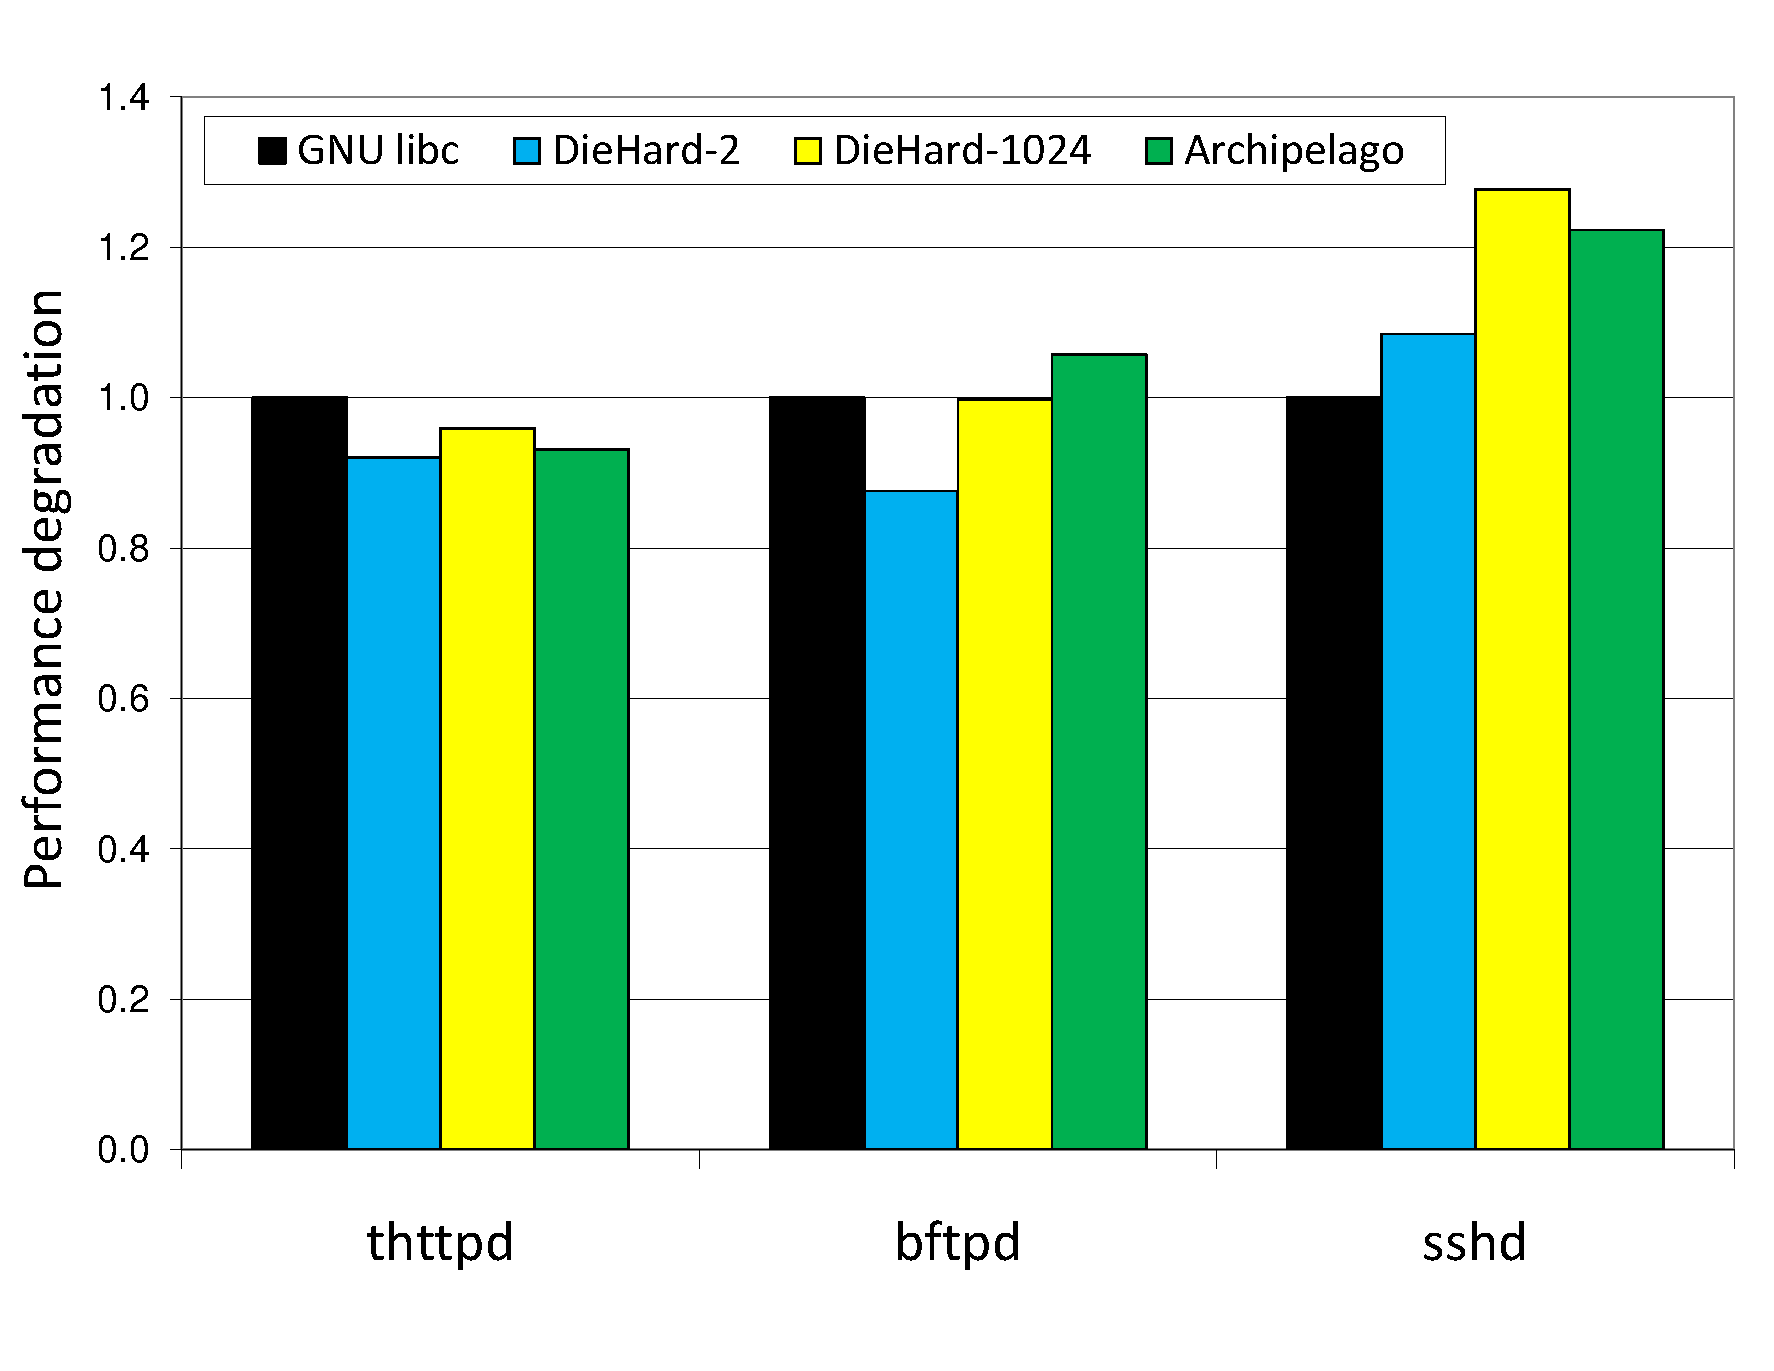
\includegraphics[width=3.25in,]{server-perf.pdf}
 \caption{Performance across a range of server applications (smaller is better), normalized to GNU libc.}
 \label{fig:runtime}
\end{figure}



\subsection{Space Overhead}


\label{sec:eval-memory}

\noindent
We evaluate the additional memory consumption incurred by using
Archipelago, and compare this to DieHard and GNU libc.
% use two different multipliers for the DieHard
%experiments.  For reference purposes, we include memory consumption of
%all the servers running with GNU libc as well.

Figure~\ref{fig:virtual} shows virtual memory consumption of three
different servers in our experiments. Due to the fact that Archipelago
preallocates a large memory pool at start-up, its virtual memory
consumption is always high compared to GNU libc. A large
fraction---more than 70\%---of that allocated space is never actually
committed to memory. The high memory consumption of \emph{bftpd} is
explained by the fact that it forks three processes for every
connected client. In our experiments, we use 50 simultaneous clients,
and measure the total memory used by all \emph{bftpd} processes, which
includes the overheads of Archipelago in each \emph{bftpd} process.

Figures~\ref{fig:memory}~and~\ref{fig:pressure} show resident memory
consumption of \emph{thttpd}, \emph{bftpd}, and \emph{sshd} during our
experiments without and with memory pressure, respectively. We
simulate memory pressure by locking pages in memory so that only about
512MB is usable by the entire system. Our experiments show that
Archipelago uses less memory than DieHard-1024 and uses on average 3
to 5 times as much memory as GNU libc. This number is much lower for
\emph{thttpd} and \emph{sshd}, which do not spawn multiple
processes. It is important to note that memory consumption with
Archipelago in the absence of memory pressure is artificially inflated,
because Linux reclaims available pages only under memory pressure.

\begin{figure}[t]
 \centering
 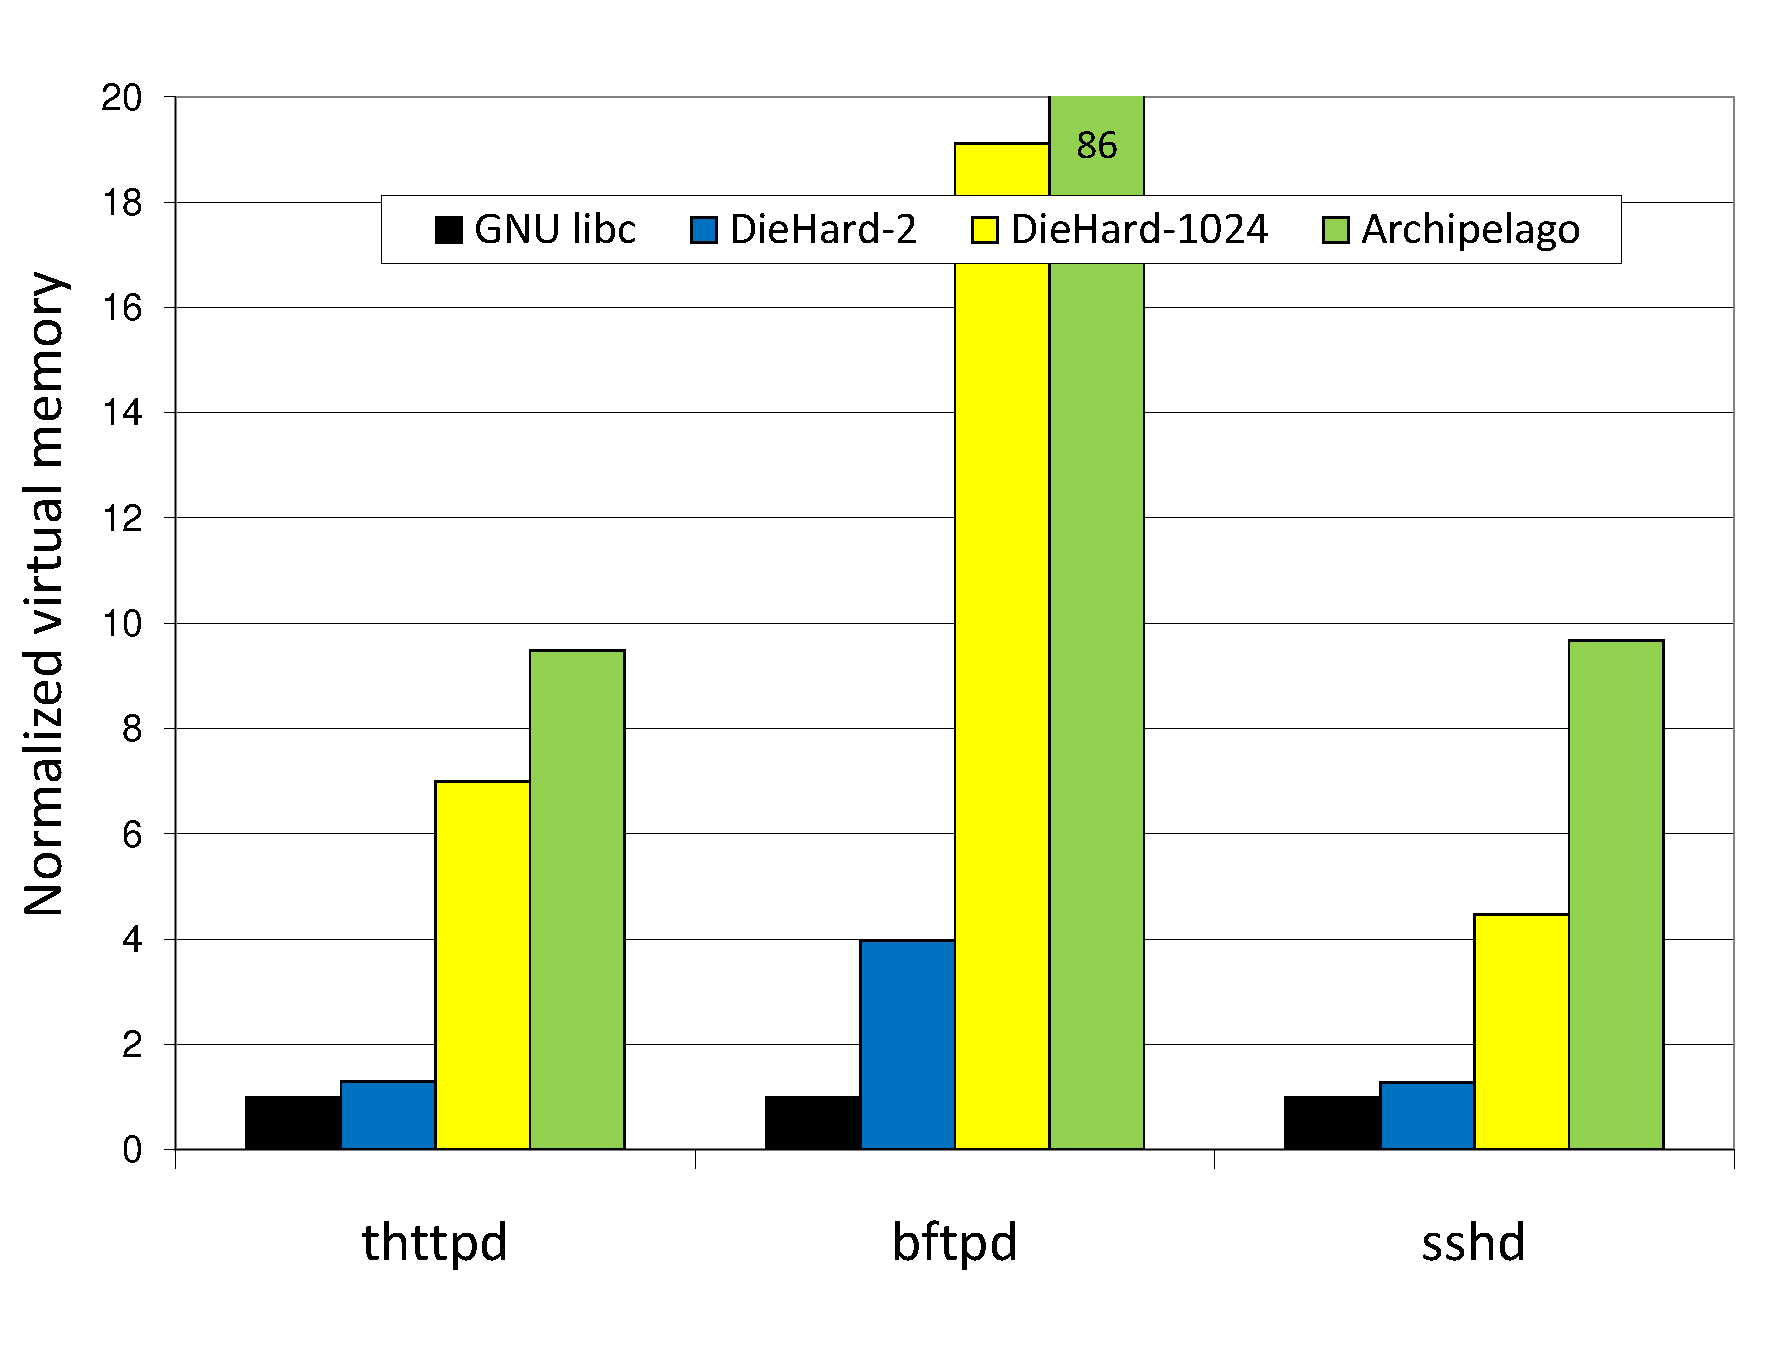
\includegraphics[width=3.25in]{vm-usage.pdf}
 \caption{Virtual memory usage of GNU libc, DieHard, and Archipelago, across a range of server applications.}
 \label{fig:virtual}
\end{figure}

\begin{figure*}[t!]
 \centering
 \subfigure[Resident memory usage, without memory pressure.\label{fig:memory}]{
 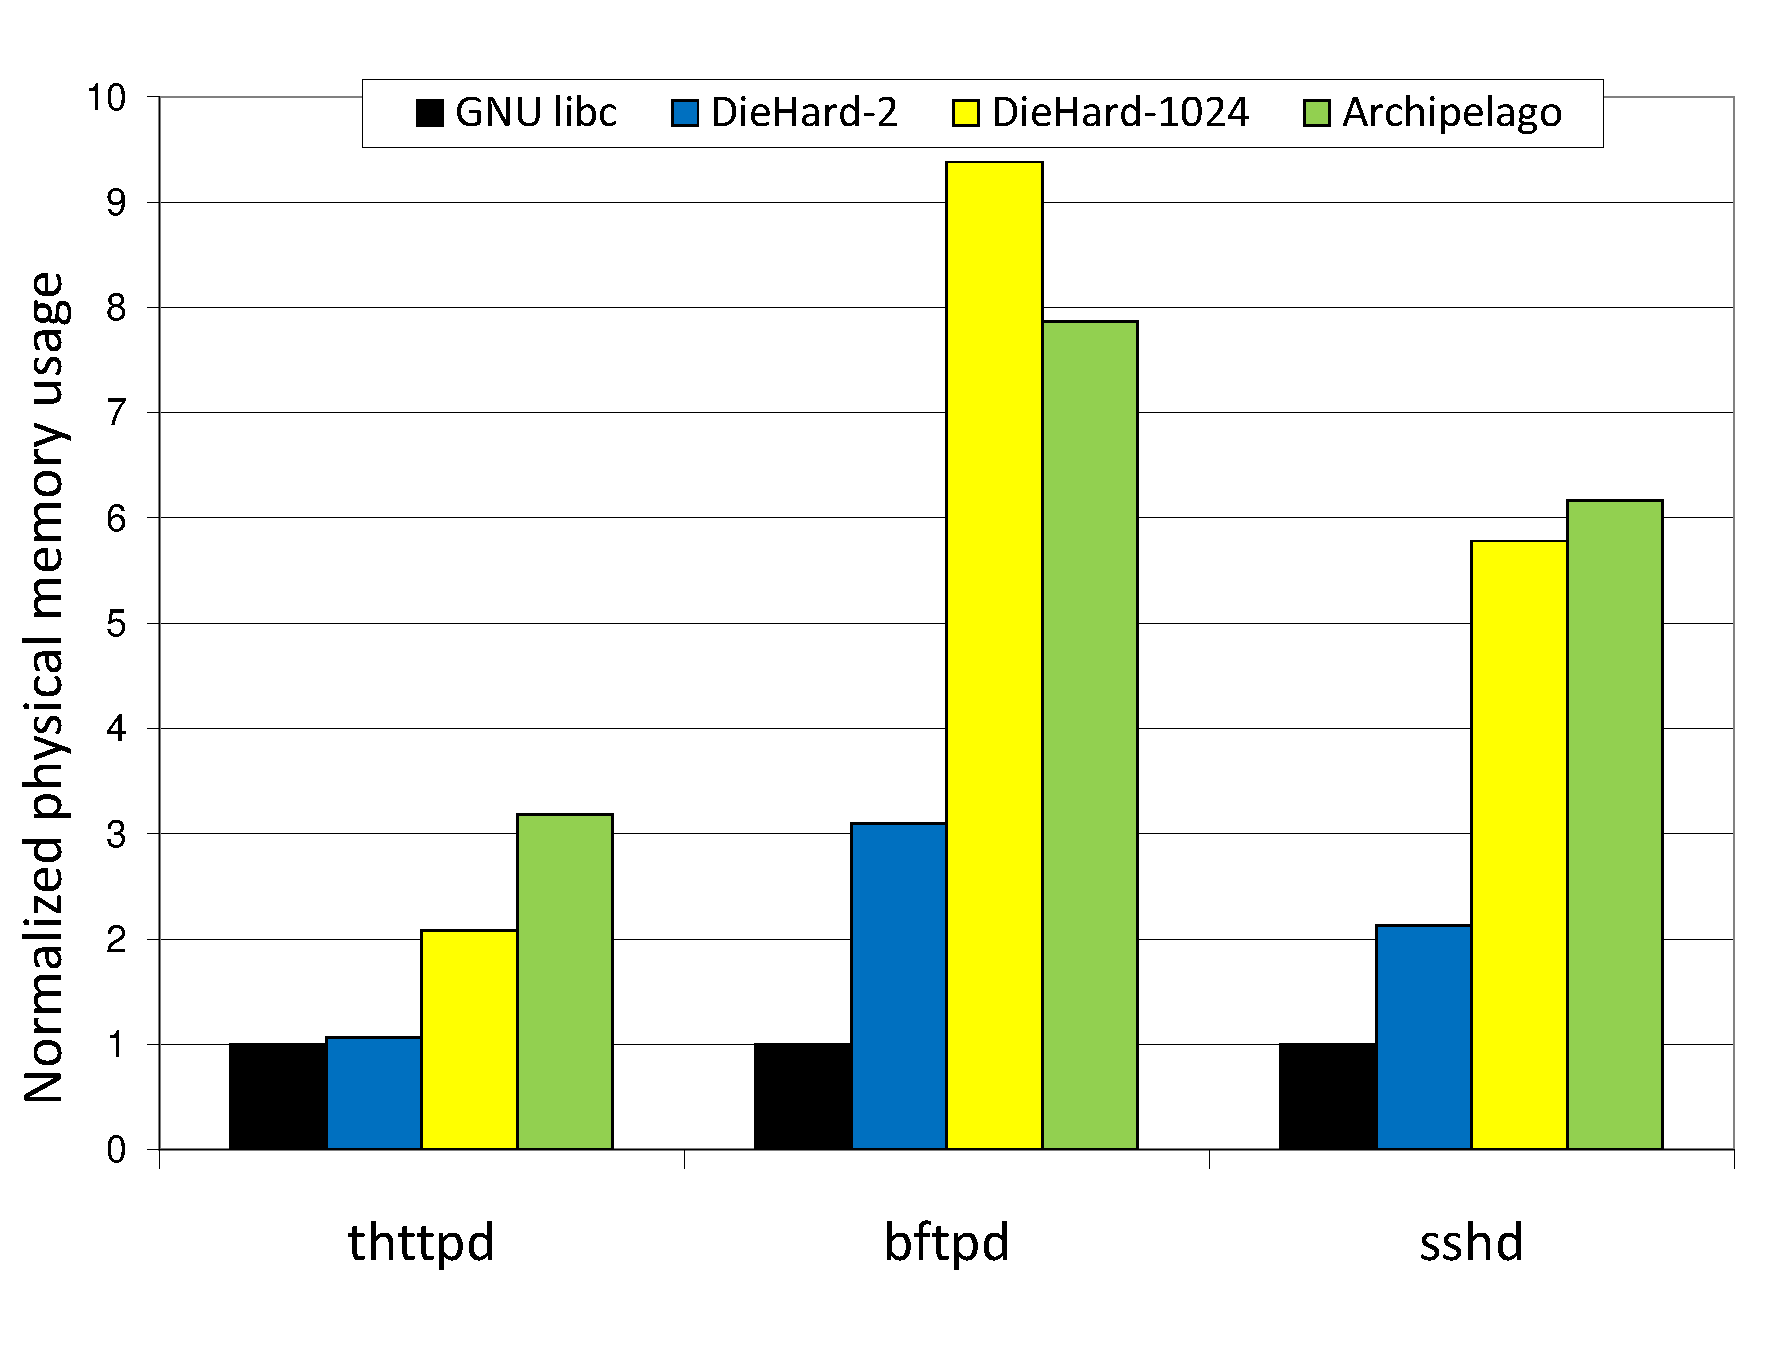
\includegraphics[width=3.25in]{rs-usage.pdf}
}\hfill
\subfigure[Resident memory usage, with memory pressure.\label{fig:pressure}]{
 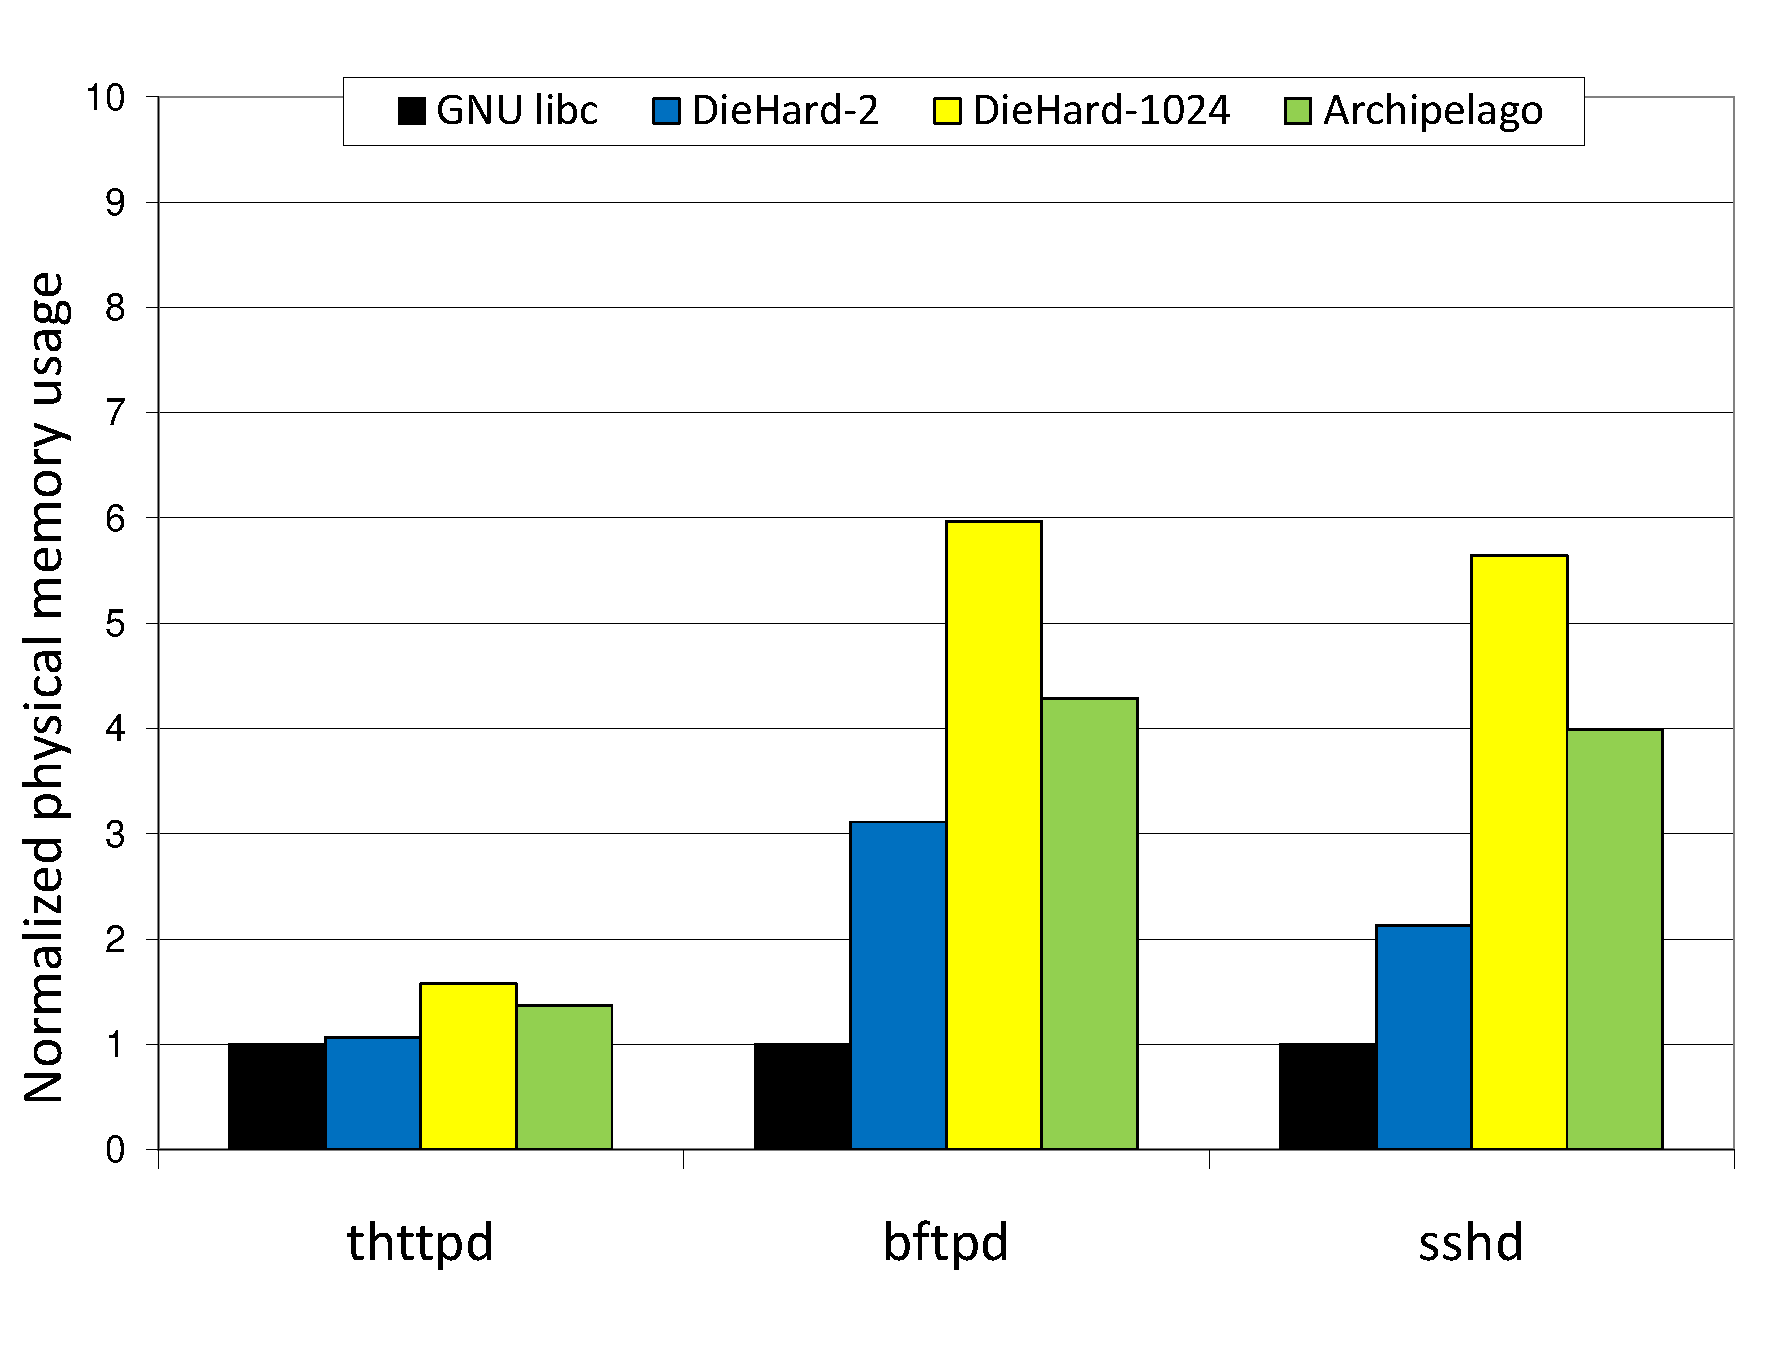
\includegraphics[width=3.25in]{rs-usage-pressure.pdf}
}
\caption{Resident memory usage with and without memory pressure. Under memory pressure, Linux quickly reclaims Archipelago's uncommitted pages, making its physical memory consumption strictly lower than with DieHard-1024.}
\end{figure*}



\subsection{Avoiding Injected Faults}

\label{sec:eval-injection}

\begin{table*}[!t]
\centering
\begin{tabular}{|lcccc|}
\hline
\multicolumn{5}{|c|}{\bf \small Injection experiments (\% correct executions)} \\
{\bf \small espresso} & {\bf \small GNU libc} & {\bf \small DieHard-2}
& {\bf \small DieHard-1024} & {\bf \small Archipelago} \\ \hline
\multicolumn{5}{|c|}{\em buffer overflows} \\
8 bytes, $p=0.01$ & 0\%                 & 29\%            & 77\%               & 100\% \\
8K, $p=0.0001$ & 0\%                 & 0\%             & 23\%               & 68\%  \\
4K, $p=0.001$  & 0\%                 & 0\%             & 2\%                & 42\%  \\
\multicolumn{5}{|c|}{\em dangling pointers} \\
5 mallocs, $p=0.01$     & 0\%                 & 8\%             & 91\%               & 29\%  \\
10 mallocs, $p=0.001$   & 0\%                 & 75\%            & 100\%              & 67\%  \\
20 mallocs, $p=0.0001$  & 0\%                 & 96\%            & 100\%              & 98\%  \\ \hline
\end{tabular}
\caption{The performance of various runtime systems in response to injected memory errors (Section~\ref{sec:eval-injection}). Archipelago provides the best protection against overflows of all sizes and frequencies, and reasonable protection against dangling pointer errors (all executions fail with GNU libc).\label{tbl:injection-errors}}
\end{table*}


\noindent
We evaluate the effectiveness of Archipelago in tackling memory errors
by using two different types of fault injectors: an overflow injector
and a dangling pointer injector. We inject faults into \emph{espresso}
running with GNU libc, DieHard and Archipelago. We perform all our
injection experiments 100 times, and record the number of times that
\emph{espresso} produces correct
output. Table~\ref{tbl:injection-errors} summarizes these results.

% EDB FIX ME We subjected these applications to an unusually large number of overflows.

{\bf Buffer overflows:} We perform three sets of experiments with the overflow injector. We
inject 8-byte overflows with 0.01 probability, 4K overflows with 0.001
probability, and 8K overflows with 0.0001 probability. These
probabilities correspond to thousands, hundreds, and tens of injected
faults, respectively.

In this set of experiments, GNU libc crashes every time, as
expected. Archipelago substantially outperforms both variants of
DieHard across the range of overflow sizes and frequencies. With small
and frequent overflows, Archipelago runs correctly every
time. DieHard-1024 does reasonably well, running correctly 77\% of the
time, while DieHard-2 only runs correctly 29\% of the time.

With large but infrequent overflows, Archipelago runs correctly 68\%
of the time. In this case, DieHard-1024 runs correctly only 23\% of
the time, while DieHard-2 crashes every time. Even in the worst case
of large and reasonably frequent overflows, Archipelago lets {\tt
espresso} run correctly 42\% of the time, while it only runs 2\% of
the time with DieHard-1024 (DieHard-2 crashes every time in this
case).

These results show that Archipelago provides excellent protection
against buffer overflows and offers dramatic improvement over DieHard,
even with an expansion factor of 1024.

{\bf Dangling pointers:} Archipelago's design goal was to limit the
impact of buffer overflows, but it also provides a measure of
protection against dangling pointers. To measure the impact of
dangling pointers on runtime systems, we injected dangling pointer
faults that free objects 5, 10 and 20 allocations early with
probabilities 0.01, 0.001 and 0.0001, respectively.

These experiments show that, as expected, DieHard-1024 offers better
protection from dangling pointer errors than Archipelago. This result
is explained by the fact that DieHard-1024 has vastly more available
object slots for reuse than Archipelago does. Archipelago has fewer
potential slots to place new objects, since it only allows one object
per page. Archipelago also instructs the operating system that all
freed objects are available for the operating system to reuse at its
discretion. If the operating system reuses a page, the original
contents will be lost, and access through a dangling pointer to this
data will trigger a fault. Nonetheless, Archipelago provides
substantial protection against these errors, running correctly 29\% of
the time in the first experiment, 67\% of the time in the second, and
98\% in the third.

\subsection{Avoiding Real Buffer Overflows}
\label{sec:eval-bug}

\noindent
To evaluate the effectiveness of Archipelago against real-life buffer
overflows, we reproduce two well-known buffer overflow-based exploits:
one in the \emph{pine} mail reader, and the other in the \emph{Squid}
web cache proxy.

We reproduce an exploit in \emph{pine} version 4.44. The exploit
is a buffer overflow that can be triggered by a maliciously formed
email message and causes \emph{pine} to crash and fail to restart
until the message is manually removed. When we place a maliciously
formed message in a user's mailbox, \emph{pine} with GNU libc crashes
whenever the user attempts to open a mailbox. However, when running
with Archipelago, \emph{pine} successfully opens the mailbox and
performs all standard operations with messages in it, including the
malicious message, without any user-noticeable slowdown.

We also test Archipelago's ability to withstand a heap buffer overflow for the
\emph{squid} web cache. For version 2.3.STABLE5, a maliciously formed request causes
a buffer overflow that corrupts heap meta-data (this causes GNU libc
to terminate). When running with Archipelago, \emph{squid}
consistently handles the malicious request correctly, without
crashing.

% EDB FIX ME Add correct ref for Valgrind (PLDI 2007)!

\section{Overflow Detection}
\label{sec:efence}

\noindent
Archipelago not only lets programs to run in the face of memory
errors, but can also be used to detect and report these
errors. Archipelago detects these errors using three separate
approaches. First, Archipelago clears all memory pool pages before
their first use. Because every page is initialized to zero, any
non-zero value past the end of an object's allocated space indicates
an overflow. Archipelago scans the contents of a page past an
allocated object on every {\tt free}.

Second, Archipelago piggybacks buffer overflow detection onto page
compaction, letting it discover overflows before an object is
deallocated. Whenever a page is compacted, Archipelago recomputes the
actual size of the object on that page by scanning it backwards until
the first non-zero word. As above, any non-zero past the end indicates
an overflow.

Finally, if an overflow touches a protected or unmapped page,
Archipelago reports this as a heap overflow.

\newpage

\subsection{Evaluation}

\noindent
To evaluate Archipelago's buffer overflow detection, we compare it to
Valgrind (using the Memcheck tool~\cite{Sew:memcheck2005}) and
Electric Fence~\cite{efence}. These tools differ substantially from
Archipelago in their approaches. Valgrind uses heavyweight dynamic
binary instrumentation to insert run-time checks; the Memcheck tool
detects a wide range of memory errors (not just heap overflows)
throughout program execution. Electric Fence is a debugging allocator
that, like Archipelago, allocates heap objects on separate pages. It
allocates three pages for every object: one page for the object itself
(placed at the end), and a memory-protected page before and after the
object. Electric Fence aborts whenever an overflow causes a memory
protection fault.

We measure Archipelago's overhead in overflow detection mode by
running \emph{espresso}, which effectively measures its worst-case
performance. Archipelago is more efficient than Electric Fence (10.5x
faster) and Valgrind (4.65x faster).

We then ran all three tools on \emph{pine}, attempting to detect the
buffer overflow we exploit in Section~\ref{sec:eval-bug}. Both
Electric Fence and Valgrind successfully detect a single buffer
overflow, but then abort the computation. However, Archipelago allows
\emph{pine} to safely continue execution and detects a second overflow. 
This experiment demonstrates Archipelago's advantage over other tools:
it can detect \emph{multiple} heap overflows in a single run.

%Since Archipelago detects buffer overflows
%only during compaction, the maximum working set size has to be
%small. In our experiments, we set it to 500 objects. Also, detecting
%actual buffer overflows requires that pages from the memory pool be
%cleared before reuse. Otherwise, Archipelago would report a large
%number of false positives, because it confuses leftover non-zero data
%from freed objects with results of out-of-bound writes. Normally, we
%do not clear the pages in the interests of performance, but in this
%set of experiments, we do. In our experiments with \emph{espresso},
%Electric Fence was 3.17 times slower, and Valgrind was 1.4 times
%slower than Archipelago in overflow-detecting mode.

\section{Related Work}



\label{sec:related}

\noindent
This section first discusses past work that exploits large address
spaces, and then describes related work in the spheres of memory
management, fault tolerance, and software engineering that address the
problem of memory errors in C/C++ programs.

The advent of 64-bit processors sparked research in operating systems
designed for large address spaces~\cite{chase94opal}.  Druschel and
Peterson point out that this address space is sufficiently large that it
can be used to provide high performance protection and security by
hiding processes from each other~\cite{druschel92hiding}.  Anonymous
RPC (ARPC) uses random placement of processes in a large address space
to eliminate expensive hardware context switches on cross-domain
RPC calls~\cite{yarvin93usenix}.  We are also leveraging a large
address space, but instead of using the space to protect independent
processes from each other, we are isolating individual objects from
memory errors within the same process.

%{\bf Large address spaces:}

%{\bf FIX ME discuss Opal.} {\bf Anonymous RPC:
%Low-Latency Protection in a 64-Bit Address Space
% Curtis Yarvin, Richard Bukowski, and Thomas Anderson}. http://citeseer.ist.psu.edu/34418.html {\bf Fbufs: A High-Bandwidth Cross-Domain Transfer Facility}.

% {\bf FIX ME: trade-off -- higher reliability, acceptable perf
% overhead.} 

Archipelago builds on the ideas of Berger and Zorn's DieHard
system~\cite{1134000}. Like DieHard, Archipelago uses a randomized
memory manager to provide protection from buffer overflows and
dangling pointer errors.  Unlike DieHard, Archipelago achieves high
reliability by dramatically increasing the size of the address space
and does not use replication.  By exploiting both standard OS
mechanisms and common program behavior, Archipelago provides greater
resilience to buffer overflow errors with moderate and acceptable CPU
and memory overhead.

Exterminator is another runtime system that, like DieHard, is based on
randomized, overprovisioned heaps~\cite{novark07exterminator}.  The
focus of Exterminator is on automatic error detection and correction
based on accumulating data from multiple executions.  While
Archipelago can also be used for overflow detection, it is closer in
spirit to DieHard, and unlike Exterminator, provides greater error
tolerance without the requirement that errors first be detected.

A number of compiler-assisted approaches have been introduced to
combat memory errors. Semantics provided by Archipelago to programs
containing buffer overflows are similar to those of Rinard et al.'s
Boundless Memory Blocks~\cite{rinard04dynamic}. Because Boundless
Memory Blocks uses a fixed-size LRU cache to store the values of
out-of-bounds writes, accesses to out-of-bounds addresses are undefined
if the object has been evicted from the cache. A number of other
unsound approaches have been proposed~\cite{dhur03,failure-oblivious}.
Dhurjati et al. use pool allocation to provide an efficient form of
memory safety that guarantees that structure fields are referenced
with the correct type.  While they guarantee type-safety, there is no
guarantee that the object the programmer had intended to access is
correctly accessed~\cite{dhur03}.  Unlike this previous work,
Archipelago provides a strong, quantifiable probabilistic guarantee
that the intended program behavior will be preserved.

%{\bf FIX ME: Dhurjati -- type-safe but unsound.} 
% {\bf FIX ME: SAFEcode}

More traditional safe-C compilers~\cite{swamy05experience, 503286,
cred} use modified versions of C and some combination of static
analysis and dynamic checks to provide protection from memory
errors. Cyclone~\cite{713871, swamy05experience} augments C with an
advanced type system to provide safe explicit memory
management. CCured~\cite{503286} inserts dynamic checks that ensure
safety into the compiled program and uses static analysis to eliminate
checks from places where memory errors cannot occur. CRED~\cite{cred}
only targets string buffer overflows, and inserts dynamic checks on
memory accesses that use out-of-bounds pointers. All of these
techniques are aimed at detecting memory errors and terminating the
program in response. Archipelago, on the other hand, is aimed at
avoiding memory errors and allowing the program to continue running
correctly.

Like Archipelago, Rx can help avoid memory errors~\cite{rx}. It
performs periodic checkpointing of program execution, and when an
error occurs, it re-runs the program from a checkpoint in a modified
environment. In response to crashes, Rx pads allocations to avoid
buffer overflows, and delays reuse of freed memory to prevent dangling
pointers. Two fundamental limitations of Rx are that it only works
with applications that allow replay, and cannot cope with errors that
do not result in crashes. Archipelago does not suffer from either of
these limitations.

Dangling pointer errors have been addressed in several ways in
previous work.  Dhurjati et al. employ a clever use of virtual memory
page mapping and protection to allow them to detect dangling pointers
at low cost~\cite{dhurjati06}.  While Archipelago also uses virtual
memory protection, our focus is on providing resilience to buffer
overflows with less emphasis on dangling pointers.  Garbage collection
is an alternative runtime system that provides safety from dangling
pointer errors. The most commonly used garbage collector for C
programs is Boehm-Demers-Weiser conservative garbage
collector~\cite{boeh88}.  Unlike Archipelago, garbage collection
provides no protection against buffer overflow errors. Garbage
collection also imposes significant space and time overheads to
achieve reasonable performance~\cite{hert05a}.

% {\bf EDB FIX ME connect to Arch overheads, cite self.}

Finally, a number of testing tools and debugging
allocators~\cite{1168884,pageheap,efence} can aid programmers in
debugging memory
errors. Valgrind~\cite{Net:bounds-checking2004,Sew:memcheck2005} and
Purify~\cite{Hastings:91} use binary instrumentation or emulation to
detect memory errors at runtime. They typically incur prohibitively
high overhead both in terms of performance (up to 25X) and space
(10X), making them only suitable during testing. Electric
Fence~\cite{efence} uses page protection to detect buffer overflow and
dangling pointer errors. As we show in section~\ref{sec:efence},
Electric Fence incurs high performance overhead and memory overhead,
especially when used to detect dangling pointer errors. Unlike both of
these systems, Archipelago can detect multiple heap buffer overflows
in a single execution.

% {\bf FIX ME - results off? Discuss Arch results here?}


\section{Future Work}
\label{sec:future}

There are a number of ways that the current Archipelago implementation
can be improved.  We intend to explore adaptively sizing the memory
pool size to achieve the optimal trade-off between performance
overhead and resilience to errors.  Our current implementation has a
static FIFO size, and we intend to investigate techniques to grow and
shrink the FIFO size just as an OS virtual memory manager adapts
working set size.  Because our approach uses very large virtual
address spaces with sparsely mapped pages, we will investigate how OS
support for sparse page tables can improve Archipelago performance.
Hardware TLBs have remained relatively small despite enormous growth
in physical memory sizes over the last two decades.  We anticipate
that TLB designs that better accomodate large sparse virtual memories,
such as those proposed by Huck and Hays~\cite{huck93isca}, will significantly
benefit Archipelago's performance.

% Adaptive hot set FIFO size, adaptive pool size, better operating
% system support for sparse page tables. Hardware support for larger
% TLBs, experiments on systems with multilevel TLB, such as the PowerPC.
% Huck and Hays 1993 ``that better accomodate large, sparse virtual
% memories'' (according to Opal paper).

% NOTE: Opal stuff important cite for Grace.

\section{Conclusion}


\noindent
\label{sec:fin}
Archipelago is a runtime system that provides protection from memory
errors for unmodified C programs. It provides probabilistic protection
from both buffer overflows and dangling pointer errors with high
probability. Archipelago spreads objects far apart in the address space
and randomizes the choice of freed objects to reuse, giving
applications an illusion of infinite-size heap and protecting them
from memory errors. It leverages the virtual memory subsystem of the
underlying OS to efficiently provide a high level of memory safety to
target programs at low cost.

We show analytically and empirically that Archipelago increases the
resilience of programs to memory errors. Our
evaluation shows that Archipelago is effective against real
and injected memory errors. We show that it allows programs to
correctly execute through hundreds and even thousands of memory
errors, which is a significant improvement over current
state-of-the-art systems. We also show how our system can be used to
debug buffer overflow errors.

We further demonstrate that the overhead of using Archipelago is more
than acceptable across a range of different server applications, both
in terms of CPU performance and memory usage. We believe Archipelago
is especially suitable for deployment in order to protect servers that
have known security vulnerabilities due to heap memory errors.

%\section{Acknowledgments}
%\label{sec:ack}
%\noindent
%The authors would like to thank Ting Yang and Gene Novark for their helpful comments. Thanks also to Shan Lu and Yuanyuan Zhou for providing us the buggy inputs for \emph{squid}, and Martin Rinard for providing us the buggy inputs for \emph{pine}.

\newpage

\bibliographystyle{abbrv}
\bibliography{clones2,gcbib,emery}


\balancecolumns

\end{document}

